% Created by tikzDevice version 0.10.1 on 2017-12-06 18:14:31
% !TEX encoding = UTF-8 Unicode
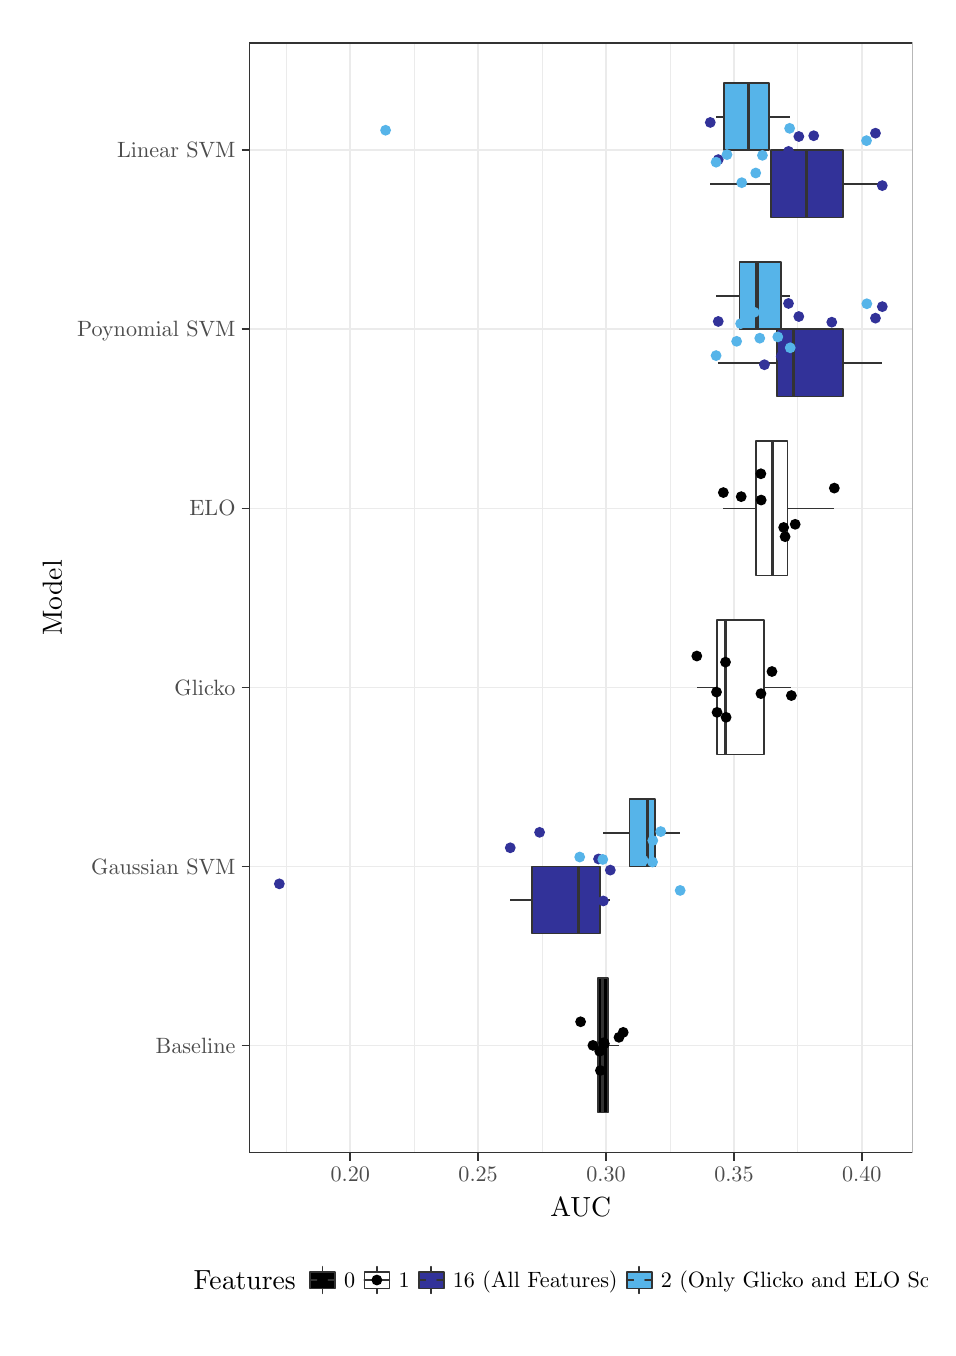
\begin{tikzpicture}[x=1pt,y=1pt]
\definecolor{fillColor}{RGB}{255,255,255}
\path[use as bounding box,fill=fillColor,fill opacity=0.00] (0,0) rectangle (325.21,469.75);
\begin{scope}
\path[clip] (  0.00,  0.00) rectangle (325.21,469.75);
\definecolor{drawColor}{RGB}{255,255,255}
\definecolor{fillColor}{RGB}{255,255,255}

\path[draw=drawColor,line width= 0.6pt,line join=round,line cap=round,fill=fillColor] (  0.00,  0.00) rectangle (325.21,469.76);
\end{scope}
\begin{scope}
\path[clip] ( 80.05, 63.15) rectangle (319.71,464.25);
\definecolor{fillColor}{RGB}{255,255,255}

\path[fill=fillColor] ( 80.05, 63.15) rectangle (319.71,464.25);
\definecolor{drawColor}{gray}{0.92}

\path[draw=drawColor,line width= 0.3pt,line join=round] ( 93.44, 63.15) --
	( 93.44,464.25);

\path[draw=drawColor,line width= 0.3pt,line join=round] (139.66, 63.15) --
	(139.66,464.25);

\path[draw=drawColor,line width= 0.3pt,line join=round] (185.88, 63.15) --
	(185.88,464.25);

\path[draw=drawColor,line width= 0.3pt,line join=round] (232.10, 63.15) --
	(232.10,464.25);

\path[draw=drawColor,line width= 0.3pt,line join=round] (278.32, 63.15) --
	(278.32,464.25);

\path[draw=drawColor,line width= 0.6pt,line join=round] ( 80.05,101.97) --
	(319.71,101.97);

\path[draw=drawColor,line width= 0.6pt,line join=round] ( 80.05,166.66) --
	(319.71,166.66);

\path[draw=drawColor,line width= 0.6pt,line join=round] ( 80.05,231.36) --
	(319.71,231.36);

\path[draw=drawColor,line width= 0.6pt,line join=round] ( 80.05,296.05) --
	(319.71,296.05);

\path[draw=drawColor,line width= 0.6pt,line join=round] ( 80.05,360.75) --
	(319.71,360.75);

\path[draw=drawColor,line width= 0.6pt,line join=round] ( 80.05,425.44) --
	(319.71,425.44);

\path[draw=drawColor,line width= 0.6pt,line join=round] (116.55, 63.15) --
	(116.55,464.25);

\path[draw=drawColor,line width= 0.6pt,line join=round] (162.77, 63.15) --
	(162.77,464.25);

\path[draw=drawColor,line width= 0.6pt,line join=round] (208.99, 63.15) --
	(208.99,464.25);

\path[draw=drawColor,line width= 0.6pt,line join=round] (255.21, 63.15) --
	(255.21,464.25);

\path[draw=drawColor,line width= 0.6pt,line join=round] (301.43, 63.15) --
	(301.43,464.25);
\definecolor{drawColor}{gray}{0.20}

\path[draw=drawColor,line width= 0.6pt,line join=round] (209.70,101.97) -- (213.67,101.97);

\path[draw=drawColor,line width= 0.6pt,line join=round] (206.07,101.97) -- (204.25,101.97);
\definecolor{fillColor}{RGB}{0,0,0}

\path[draw=drawColor,line width= 0.6pt,line join=round,line cap=round,fill=fillColor] (209.70, 77.71) --
	(206.07, 77.71) --
	(206.07,126.23) --
	(209.70,126.23) --
	(209.70, 77.71) --
	cycle;

\path[draw=drawColor,line width= 1.1pt,line join=round] (207.56, 77.71) -- (207.56,126.23);

\path[draw=drawColor,line width= 0.6pt,line join=round] (206.71,154.53) -- (210.53,154.53);

\path[draw=drawColor,line width= 0.6pt,line join=round] (182.33,154.53) -- (174.38,154.53);
\definecolor{fillColor}{RGB}{50,50,153}

\path[draw=drawColor,line width= 0.6pt,line join=round,line cap=round,fill=fillColor] (206.71,142.40) --
	(182.33,142.40) --
	(182.33,166.66) --
	(206.71,166.66) --
	(206.71,142.40) --
	cycle;

\path[draw=drawColor,line width= 1.1pt,line join=round] (198.89,142.40) -- (198.89,166.66);

\path[draw=drawColor,line width= 0.6pt,line join=round] (226.61,178.79) -- (235.77,178.79);

\path[draw=drawColor,line width= 0.6pt,line join=round] (217.50,178.79) -- (207.83,178.79);
\definecolor{fillColor}{RGB}{86,180,233}

\path[draw=drawColor,line width= 0.6pt,line join=round,line cap=round,fill=fillColor] (226.61,166.66) --
	(217.50,166.66) --
	(217.50,190.92) --
	(226.61,190.92) --
	(226.61,166.66) --
	cycle;

\path[draw=drawColor,line width= 1.1pt,line join=round] (224.11,166.66) -- (224.11,190.92);

\path[draw=drawColor,line width= 0.6pt,line join=round] (265.97,231.36) -- (275.96,231.36);

\path[draw=drawColor,line width= 0.6pt,line join=round] (249.06,231.36) -- (241.79,231.36);
\definecolor{fillColor}{RGB}{255,255,255}

\path[draw=drawColor,line width= 0.6pt,line join=round,line cap=round,fill=fillColor] (265.97,207.10) --
	(249.06,207.10) --
	(249.06,255.62) --
	(265.97,255.62) --
	(265.97,207.10) --
	cycle;

\path[draw=drawColor,line width= 1.1pt,line join=round] (252.27,207.10) -- (252.27,255.62);

\path[draw=drawColor,line width= 0.6pt,line join=round] (274.60,296.05) -- (291.48,296.05);

\path[draw=drawColor,line width= 0.6pt,line join=round] (263.17,296.05) -- (251.39,296.05);

\path[draw=drawColor,line width= 0.6pt,line join=round,line cap=round,fill=fillColor] (274.60,271.79) --
	(263.17,271.79) --
	(263.17,320.31) --
	(274.60,320.31) --
	(274.60,271.79) --
	cycle;

\path[draw=drawColor,line width= 1.1pt,line join=round] (269.12,271.79) -- (269.12,320.31);

\path[draw=drawColor,line width= 0.6pt,line join=round] (294.51,348.62) -- (308.81,348.62);

\path[draw=drawColor,line width= 0.6pt,line join=round] (270.78,348.62) -- (249.54,348.62);
\definecolor{fillColor}{RGB}{50,50,153}

\path[draw=drawColor,line width= 0.6pt,line join=round,line cap=round,fill=fillColor] (294.51,336.48) --
	(270.78,336.48) --
	(270.78,360.75) --
	(294.51,360.75) --
	(294.51,336.48) --
	cycle;

\path[draw=drawColor,line width= 1.1pt,line join=round] (276.79,336.48) -- (276.79,360.75);

\path[draw=drawColor,line width= 0.6pt,line join=round] (272.17,372.88) -- (275.54,372.88);

\path[draw=drawColor,line width= 0.6pt,line join=round] (257.25,372.88) -- (248.75,372.88);
\definecolor{fillColor}{RGB}{86,180,233}

\path[draw=drawColor,line width= 0.6pt,line join=round,line cap=round,fill=fillColor] (272.17,360.75) --
	(257.25,360.75) --
	(257.25,385.01) --
	(272.17,385.01) --
	(272.17,360.75) --
	cycle;

\path[draw=drawColor,line width= 1.1pt,line join=round] (263.54,360.75) -- (263.54,385.01);

\path[draw=drawColor,line width= 0.6pt,line join=round] (294.51,413.31) -- (308.81,413.31);

\path[draw=drawColor,line width= 0.6pt,line join=round] (268.58,413.31) -- (246.65,413.31);
\definecolor{fillColor}{RGB}{50,50,153}

\path[draw=drawColor,line width= 0.6pt,line join=round,line cap=round,fill=fillColor] (294.51,401.18) --
	(268.58,401.18) --
	(268.58,425.44) --
	(294.51,425.44) --
	(294.51,401.18) --
	cycle;

\path[draw=drawColor,line width= 1.1pt,line join=round] (281.33,401.18) -- (281.33,425.44);

\path[draw=drawColor,line width= 0.6pt,line join=round] (267.96,437.57) -- (275.33,437.57);

\path[draw=drawColor,line width= 0.6pt,line join=round] (251.70,437.57) -- (248.75,437.57);
\definecolor{fillColor}{RGB}{86,180,233}

\path[draw=drawColor,line width= 0.6pt,line join=round,line cap=round,fill=fillColor] (267.96,425.44) --
	(251.70,425.44) --
	(251.70,449.70) --
	(267.96,449.70) --
	(267.96,425.44) --
	cycle;

\path[draw=drawColor,line width= 1.1pt,line join=round] (260.56,425.44) -- (260.56,449.70);
\definecolor{fillColor}{RGB}{0,0,0}

\path[fill=fillColor] (199.80,110.53) circle (  1.96);

\path[fill=fillColor] (208.16,102.96) circle (  1.96);

\path[fill=fillColor] (204.25,101.99) circle (  1.96);

\path[fill=fillColor] (208.38,102.58) circle (  1.96);

\path[fill=fillColor] (206.69, 99.87) circle (  1.96);

\path[fill=fillColor] (215.20,106.70) circle (  1.96);

\path[fill=fillColor] (213.67,104.91) circle (  1.96);

\path[fill=fillColor] (206.96, 92.92) circle (  1.96);

\path[fill=fillColor] (257.83,300.28) circle (  1.96);

\path[fill=fillColor] (273.69,285.82) circle (  1.96);

\path[fill=fillColor] (251.38,301.76) circle (  1.96);

\path[fill=fillColor] (265.05,299.05) circle (  1.96);

\path[fill=fillColor] (277.34,290.29) circle (  1.96);

\path[fill=fillColor] (273.17,289.15) circle (  1.96);

\path[fill=fillColor] (264.94,308.55) circle (  1.96);

\path[fill=fillColor] (291.48,303.37) circle (  1.96);
\definecolor{fillColor}{RGB}{50,50,153}

\path[fill=fillColor] (206.28,169.36) circle (  1.96);

\path[fill=fillColor] (208.01,154.19) circle (  1.96);

\path[fill=fillColor] (202.52,164.14) circle (  1.96);

\path[fill=fillColor] (174.38,173.40) circle (  1.96);

\path[fill=fillColor] (184.98,178.98) circle (  1.96);

\path[fill=fillColor] (210.54,165.34) circle (  1.96);

\path[fill=fillColor] (195.27,160.36) circle (  1.96);

\path[fill=fillColor] ( 90.94,160.37) circle (  1.96);
\definecolor{fillColor}{RGB}{86,180,233}

\path[fill=fillColor] (228.75,179.26) circle (  1.96);

\path[fill=fillColor] (235.77,157.99) circle (  1.96);

\path[fill=fillColor] (220.74,175.66) circle (  1.96);

\path[fill=fillColor] (222.42,168.87) circle (  1.96);

\path[fill=fillColor] (199.48,170.06) circle (  1.96);

\path[fill=fillColor] (225.89,176.03) circle (  1.96);

\path[fill=fillColor] (225.80,168.24) circle (  1.96);

\path[fill=fillColor] (207.82,169.19) circle (  1.96);
\definecolor{fillColor}{RGB}{0,0,0}

\path[fill=fillColor] (249.11,222.34) circle (  1.96);

\path[fill=fillColor] (252.16,240.48) circle (  1.96);

\path[fill=fillColor] (241.79,242.69) circle (  1.96);

\path[fill=fillColor] (275.96,228.41) circle (  1.96);

\path[fill=fillColor] (268.94,237.09) circle (  1.96);

\path[fill=fillColor] (248.91,229.67) circle (  1.96);

\path[fill=fillColor] (264.97,229.10) circle (  1.96);

\path[fill=fillColor] (252.37,220.55) circle (  1.96);
\definecolor{fillColor}{RGB}{50,50,153}

\path[fill=fillColor] (290.58,420.30) circle (  1.96);

\path[fill=fillColor] (246.66,435.50) circle (  1.96);

\path[fill=fillColor] (274.94,425.04) circle (  1.96);

\path[fill=fillColor] (249.54,422.07) circle (  1.96);

\path[fill=fillColor] (278.66,430.42) circle (  1.96);

\path[fill=fillColor] (284.03,430.70) circle (  1.96);

\path[fill=fillColor] (306.35,431.62) circle (  1.96);

\path[fill=fillColor] (308.81,412.68) circle (  1.96);
\definecolor{fillColor}{RGB}{86,180,233}

\path[fill=fillColor] (258.03,413.73) circle (  1.96);

\path[fill=fillColor] (275.33,433.37) circle (  1.96);

\path[fill=fillColor] (263.08,417.23) circle (  1.96);

\path[fill=fillColor] (129.33,432.68) circle (  1.96);

\path[fill=fillColor] (248.76,421.14) circle (  1.96);

\path[fill=fillColor] (252.70,423.88) circle (  1.96);

\path[fill=fillColor] (265.50,423.61) circle (  1.96);

\path[fill=fillColor] (303.11,428.92) circle (  1.96);
\definecolor{fillColor}{RGB}{50,50,153}

\path[fill=fillColor] (278.65,365.37) circle (  1.96);

\path[fill=fillColor] (249.54,363.59) circle (  1.96);

\path[fill=fillColor] (290.56,363.32) circle (  1.96);

\path[fill=fillColor] (274.92,370.09) circle (  1.96);

\path[fill=fillColor] (272.30,350.95) circle (  1.96);

\path[fill=fillColor] (308.82,368.94) circle (  1.96);

\path[fill=fillColor] (266.23,347.95) circle (  1.96);

\path[fill=fillColor] (306.35,364.78) circle (  1.96);
\definecolor{fillColor}{RGB}{86,180,233}

\path[fill=fillColor] (262.57,366.91) circle (  1.96);

\path[fill=fillColor] (257.62,362.80) circle (  1.96);

\path[fill=fillColor] (275.55,354.07) circle (  1.96);

\path[fill=fillColor] (303.23,369.98) circle (  1.96);

\path[fill=fillColor] (264.54,357.54) circle (  1.96);

\path[fill=fillColor] (248.76,351.25) circle (  1.96);

\path[fill=fillColor] (271.06,358.00) circle (  1.96);

\path[fill=fillColor] (256.18,356.41) circle (  1.96);

\path[draw=drawColor,line width= 0.6pt,line join=round,line cap=round] ( 80.05, 63.15) rectangle (319.71,464.25);
\end{scope}
\begin{scope}
\path[clip] (  0.00,  0.00) rectangle (325.21,469.75);
\definecolor{drawColor}{gray}{0.30}

\node[text=drawColor,anchor=base east,inner sep=0pt, outer sep=0pt, scale=  0.80] at ( 75.10, 99.22) {Baseline};

\node[text=drawColor,anchor=base east,inner sep=0pt, outer sep=0pt, scale=  0.80] at ( 75.10,163.91) {Gaussian SVM};

\node[text=drawColor,anchor=base east,inner sep=0pt, outer sep=0pt, scale=  0.80] at ( 75.10,228.60) {Glicko};

\node[text=drawColor,anchor=base east,inner sep=0pt, outer sep=0pt, scale=  0.80] at ( 75.10,293.30) {ELO};

\node[text=drawColor,anchor=base east,inner sep=0pt, outer sep=0pt, scale=  0.80] at ( 75.10,357.99) {Poynomial SVM};

\node[text=drawColor,anchor=base east,inner sep=0pt, outer sep=0pt, scale=  0.80] at ( 75.10,422.68) {Linear SVM};
\end{scope}
\begin{scope}
\path[clip] (  0.00,  0.00) rectangle (325.21,469.75);
\definecolor{drawColor}{gray}{0.20}

\path[draw=drawColor,line width= 0.6pt,line join=round] ( 77.30,101.97) --
	( 80.05,101.97);

\path[draw=drawColor,line width= 0.6pt,line join=round] ( 77.30,166.66) --
	( 80.05,166.66);

\path[draw=drawColor,line width= 0.6pt,line join=round] ( 77.30,231.36) --
	( 80.05,231.36);

\path[draw=drawColor,line width= 0.6pt,line join=round] ( 77.30,296.05) --
	( 80.05,296.05);

\path[draw=drawColor,line width= 0.6pt,line join=round] ( 77.30,360.75) --
	( 80.05,360.75);

\path[draw=drawColor,line width= 0.6pt,line join=round] ( 77.30,425.44) --
	( 80.05,425.44);
\end{scope}
\begin{scope}
\path[clip] (  0.00,  0.00) rectangle (325.21,469.75);
\definecolor{drawColor}{gray}{0.20}

\path[draw=drawColor,line width= 0.6pt,line join=round] (116.55, 60.40) --
	(116.55, 63.15);

\path[draw=drawColor,line width= 0.6pt,line join=round] (162.77, 60.40) --
	(162.77, 63.15);

\path[draw=drawColor,line width= 0.6pt,line join=round] (208.99, 60.40) --
	(208.99, 63.15);

\path[draw=drawColor,line width= 0.6pt,line join=round] (255.21, 60.40) --
	(255.21, 63.15);

\path[draw=drawColor,line width= 0.6pt,line join=round] (301.43, 60.40) --
	(301.43, 63.15);
\end{scope}
\begin{scope}
\path[clip] (  0.00,  0.00) rectangle (325.21,469.75);
\definecolor{drawColor}{gray}{0.30}

\node[text=drawColor,anchor=base,inner sep=0pt, outer sep=0pt, scale=  0.80] at (116.55, 52.69) {0.20};

\node[text=drawColor,anchor=base,inner sep=0pt, outer sep=0pt, scale=  0.80] at (162.77, 52.69) {0.25};

\node[text=drawColor,anchor=base,inner sep=0pt, outer sep=0pt, scale=  0.80] at (208.99, 52.69) {0.30};

\node[text=drawColor,anchor=base,inner sep=0pt, outer sep=0pt, scale=  0.80] at (255.21, 52.69) {0.35};

\node[text=drawColor,anchor=base,inner sep=0pt, outer sep=0pt, scale=  0.80] at (301.43, 52.69) {0.40};
\end{scope}
\begin{scope}
\path[clip] (  0.00,  0.00) rectangle (325.21,469.75);
\definecolor{drawColor}{RGB}{0,0,0}

\node[text=drawColor,anchor=base,inner sep=0pt, outer sep=0pt, scale=  1.00] at (199.88, 40.31) {AUC};
\end{scope}
\begin{scope}
\path[clip] (  0.00,  0.00) rectangle (325.21,469.75);
\definecolor{drawColor}{RGB}{0,0,0}

\node[text=drawColor,rotate= 90.00,anchor=base,inner sep=0pt, outer sep=0pt, scale=  1.00] at ( 12.39,263.70) {Model};
\end{scope}
\begin{scope}
\path[clip] (  0.00,  0.00) rectangle (325.21,469.75);
\definecolor{fillColor}{RGB}{255,255,255}

\path[fill=fillColor] ( 54.31,  5.50) rectangle (345.45, 28.93);
\end{scope}
\begin{scope}
\path[clip] (  0.00,  0.00) rectangle (325.21,469.75);
\definecolor{drawColor}{RGB}{0,0,0}

\node[text=drawColor,anchor=base west,inner sep=0pt, outer sep=0pt, scale=  1.00] at ( 60.00, 13.77) {Features};
\end{scope}
\begin{scope}
\path[clip] (  0.00,  0.00) rectangle (325.21,469.75);
\definecolor{fillColor}{RGB}{255,255,255}

\path[fill=fillColor] (100.50, 11.19) rectangle (112.54, 23.24);
\end{scope}
\begin{scope}
\path[clip] (  0.00,  0.00) rectangle (325.21,469.75);
\definecolor{drawColor}{gray}{0.20}

\path[draw=drawColor,line width= 0.6pt,line join=round,line cap=round] (106.52, 12.40) --
	(106.52, 14.20);

\path[draw=drawColor,line width= 0.6pt,line join=round,line cap=round] (106.52, 20.22) --
	(106.52, 22.03);
\definecolor{fillColor}{RGB}{0,0,0}

\path[draw=drawColor,line width= 0.6pt,line join=round,line cap=round,fill=fillColor] (102.00, 14.20) rectangle (111.04, 20.22);

\path[draw=drawColor,line width= 0.6pt,line join=round,line cap=round] (102.00, 17.21) --
	(111.04, 17.21);
\end{scope}
\begin{scope}
\path[clip] (  0.00,  0.00) rectangle (325.21,469.75);
\definecolor{fillColor}{RGB}{0,0,0}

\path[fill=fillColor] (106.52, 17.21) circle (  1.96);
\end{scope}
\begin{scope}
\path[clip] (  0.00,  0.00) rectangle (325.21,469.75);
\definecolor{fillColor}{RGB}{255,255,255}

\path[fill=fillColor] (120.15, 11.19) rectangle (132.20, 23.24);
\end{scope}
\begin{scope}
\path[clip] (  0.00,  0.00) rectangle (325.21,469.75);
\definecolor{drawColor}{gray}{0.20}

\path[draw=drawColor,line width= 0.6pt,line join=round,line cap=round] (126.18, 12.40) --
	(126.18, 14.20);

\path[draw=drawColor,line width= 0.6pt,line join=round,line cap=round] (126.18, 20.22) --
	(126.18, 22.03);
\definecolor{fillColor}{RGB}{255,255,255}

\path[draw=drawColor,line width= 0.6pt,line join=round,line cap=round,fill=fillColor] (121.66, 14.20) rectangle (130.69, 20.22);

\path[draw=drawColor,line width= 0.6pt,line join=round,line cap=round] (121.66, 17.21) --
	(130.69, 17.21);
\end{scope}
\begin{scope}
\path[clip] (  0.00,  0.00) rectangle (325.21,469.75);
\definecolor{fillColor}{RGB}{0,0,0}

\path[fill=fillColor] (126.18, 17.21) circle (  1.96);
\end{scope}
\begin{scope}
\path[clip] (  0.00,  0.00) rectangle (325.21,469.75);
\definecolor{fillColor}{RGB}{255,255,255}

\path[fill=fillColor] (139.81, 11.19) rectangle (151.86, 23.24);
\end{scope}
\begin{scope}
\path[clip] (  0.00,  0.00) rectangle (325.21,469.75);
\definecolor{drawColor}{gray}{0.20}

\path[draw=drawColor,line width= 0.6pt,line join=round,line cap=round] (145.83, 12.40) --
	(145.83, 14.20);

\path[draw=drawColor,line width= 0.6pt,line join=round,line cap=round] (145.83, 20.22) --
	(145.83, 22.03);
\definecolor{fillColor}{RGB}{50,50,153}

\path[draw=drawColor,line width= 0.6pt,line join=round,line cap=round,fill=fillColor] (141.32, 14.20) rectangle (150.35, 20.22);

\path[draw=drawColor,line width= 0.6pt,line join=round,line cap=round] (141.32, 17.21) --
	(150.35, 17.21);
\end{scope}
\begin{scope}
\path[clip] (  0.00,  0.00) rectangle (325.21,469.75);
\definecolor{fillColor}{RGB}{50,50,153}

\path[fill=fillColor] (145.83, 17.21) circle (  1.96);
\end{scope}
\begin{scope}
\path[clip] (  0.00,  0.00) rectangle (325.21,469.75);
\definecolor{fillColor}{RGB}{255,255,255}

\path[fill=fillColor] (214.97, 11.19) rectangle (227.01, 23.24);
\end{scope}
\begin{scope}
\path[clip] (  0.00,  0.00) rectangle (325.21,469.75);
\definecolor{drawColor}{gray}{0.20}

\path[draw=drawColor,line width= 0.6pt,line join=round,line cap=round] (220.99, 12.40) --
	(220.99, 14.20);

\path[draw=drawColor,line width= 0.6pt,line join=round,line cap=round] (220.99, 20.22) --
	(220.99, 22.03);
\definecolor{fillColor}{RGB}{86,180,233}

\path[draw=drawColor,line width= 0.6pt,line join=round,line cap=round,fill=fillColor] (216.47, 14.20) rectangle (225.51, 20.22);

\path[draw=drawColor,line width= 0.6pt,line join=round,line cap=round] (216.47, 17.21) --
	(225.51, 17.21);
\end{scope}
\begin{scope}
\path[clip] (  0.00,  0.00) rectangle (325.21,469.75);
\definecolor{fillColor}{RGB}{86,180,233}

\path[fill=fillColor] (220.99, 17.21) circle (  1.96);
\end{scope}
\begin{scope}
\path[clip] (  0.00,  0.00) rectangle (325.21,469.75);
\definecolor{drawColor}{RGB}{0,0,0}

\node[text=drawColor,anchor=base west,inner sep=0pt, outer sep=0pt, scale=  0.80] at (114.35, 14.46) {0};
\end{scope}
\begin{scope}
\path[clip] (  0.00,  0.00) rectangle (325.21,469.75);
\definecolor{drawColor}{RGB}{0,0,0}

\node[text=drawColor,anchor=base west,inner sep=0pt, outer sep=0pt, scale=  0.80] at (134.01, 14.46) {1};
\end{scope}
\begin{scope}
\path[clip] (  0.00,  0.00) rectangle (325.21,469.75);
\definecolor{drawColor}{RGB}{0,0,0}

\node[text=drawColor,anchor=base west,inner sep=0pt, outer sep=0pt, scale=  0.80] at (153.66, 14.46) {16 (All Features)};
\end{scope}
\begin{scope}
\path[clip] (  0.00,  0.00) rectangle (325.21,469.75);
\definecolor{drawColor}{RGB}{0,0,0}

\node[text=drawColor,anchor=base west,inner sep=0pt, outer sep=0pt, scale=  0.80] at (228.82, 14.46) {2 (Only Glicko and ELO Score)};
\end{scope}
\end{tikzpicture}
